\documentclass[12pt]{article}
\usepackage[utf8]{inputenc}
\usepackage{amsmath}
\usepackage[spanish,es-tabla]{babel}
\usepackage{graphicx}
\usepackage{amssymb, amsmath, amsbsy} 
\usepackage{mathtools}
\usepackage{multicol}
\usepackage{scalerel,amsmath}
\usepackage [ spanish ]{babel}
\usepackage [utf 8]{inputenc }
\usepackage {graphicx }
\usepackage[a4paper]{geometry}
\geometry{top=1.5cm, bottom=1.0cm, left=1.25cm, right=1.25cm}

\begin{document}
\graphicspath{{images/}}
	\begin{center}
	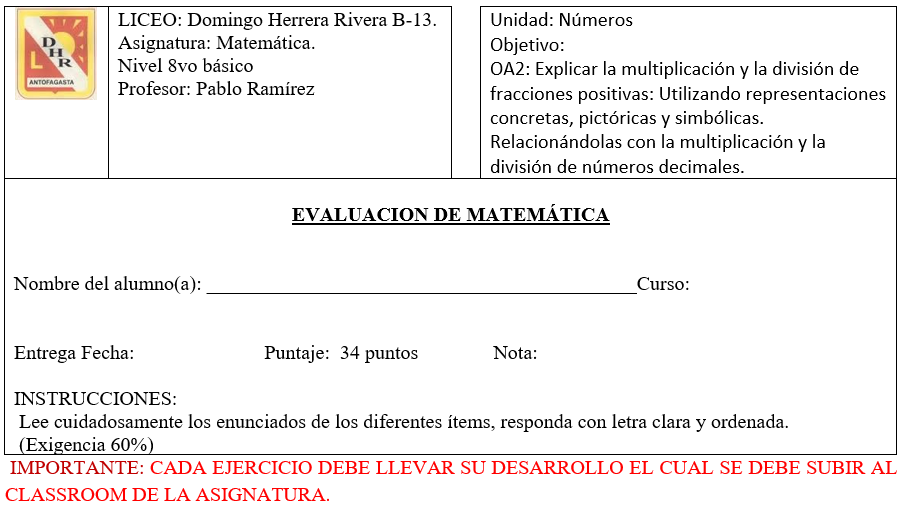
\includegraphics [ width =1.0\textwidth]{ENCABEZADO.png}\\
	\end{center} 
		\begin{enumerate}
		\item [Item I] Resuelva los siguientes ejercicios. 
	\end{enumerate}
\begin{multicols}{2}
	\begin{enumerate}
		\item [1] El resultado de $\dfrac{1}{2} \cdot \dfrac{3}{5}$	es: 
	\begin{enumerate}
	\item $\dfrac{5}{3}$\\
	\item $\dfrac{5}{6}$\\
	\item $\dfrac{3}{10}$\\
	\item $\dfrac{2}{15}$\\

\end{enumerate}
\end{enumerate}

\begin{enumerate}
\item [2]El resultado de $\dfrac{2}{5} \cdot \dfrac{15}{8}$	es:
\begin{enumerate}
	\item $\dfrac{16}{75}$\\
	\item $\dfrac{3}{4}$\\
	\item $\dfrac{30}{16}$\\
	\item $\dfrac{4}{3}$\\

\end{enumerate}
\end{enumerate}
\end{multicols}
\ \\ \
\begin{multicols}{2}
		\begin{enumerate}
		\item [3]El resultado de $\dfrac{2}{9} \cdot \dfrac{12}{2}$	es:
			\begin{enumerate}
			\item $\dfrac{12}{9}$\\
			\item $\dfrac{12}{18}$\\
			\item $\dfrac{24}{12}$\\
			\item $\dfrac{24}{15}$\\ 
	\end{enumerate}
	\end{enumerate}
\begin{enumerate}
	\item [4]El resultado de $\dfrac{9}{2} \cdot \dfrac{5}{7}$	es:
	\begin{enumerate}
		\item $\dfrac{10}{63}$\\
		\item $\dfrac{10}{9}$\\
		\item $\dfrac{18}{35}$\\
		\item $\dfrac{45}{14}$\\
	\end{enumerate}
\end{enumerate}
\end{multicols}	

\begin{multicols}{2}
   \begin{enumerate}
   	\item [5] La fracción  $\dfrac{12}{5} $	corresponde a una fracción:
   	\begin{enumerate}
   		\item fracción impropia\\
   		\item fracción propia\\
   		\item fracción decimal\\
   	\end{enumerate}
   \end{enumerate}
   \begin{enumerate}
   	\item [6] Transforme $\scalerel{5}{\dfrac{1}{3}}$ a fracción impropia: 
   	   	\begin{enumerate}
   		\item $\dfrac{16}{3}$\\
   		\item $\dfrac{15}{3}$\\
   		\item $\dfrac{3}{15}$\\
     	\end{enumerate}
   \end{enumerate} 
\end{multicols}
\begin{multicols}{2}
	\begin{enumerate}
		\item [7]El resultado de $\dfrac{2}{5} \cdot \dfrac{15}{8}$	es:
		\begin{enumerate}
			\item $\dfrac{5}{3}$\\
			\item $\dfrac{5}{6}$\\
			\item $\dfrac{3}{10}$\\
			\item $\dfrac{2}{15}$\\
		\end{enumerate}
	\end{enumerate}
\begin{enumerate}
	\item [8]El resultado de $\dfrac{2}{5} \cdot \dfrac{15}{8}$	es:
	\begin{enumerate}
		\item $\dfrac{5}{3}$\\
		\item $\dfrac{5}{6}$\\
		\item $\dfrac{3}{10}$\\
		\item $\dfrac{2}{15}$\\
	\end{enumerate}
\end{enumerate}
\end{multicols}
\begin{enumerate}
	\item [9]El resultado de $\dfrac{2}{5} \cdot \dfrac{15}{8}$	es:
	\begin{enumerate}
		\item $\dfrac{5}{3}$\\
		\item $\dfrac{5}{6}$\\
		\item $\dfrac{3}{10}$\\
		\item $\dfrac{2}{15}$\\
	\end{enumerate}
\ \\ 
%%%%item 2%%%%%
\item [Item II] Transforme los siguientes valores de decimal a fracción o de fracción a decimal, según corresponda. 
\begin{multicols}{2}
	\begin{enumerate}
		\item [10] El decimal 1,02 es igual a:
	\end{enumerate}
		\begin{enumerate}
			\item $\dfrac{102}{10}$\\
			\item $\dfrac{102}{1000}$\\
			\item $\dfrac{102}{100}$\\
			\end{enumerate}

	\begin{enumerate}
		\item [11]La fracción $\dfrac{15}{1000}$	 es equivalente a:
			\end{enumerate}
		\begin{enumerate}
			\item $0,0015$\\
			\item $0,015$\\
			\item $15,00$\\
	\end{enumerate}
\end{multicols}
\ \\ 
	\begin{enumerate}
		\item [12]El resultado de $\dfrac{1}{2} \cdot \dfrac{13}{5}$  es$^\ast$: 		\\
			\end{enumerate}
		\begin{enumerate}
			\item $1,3$\\
			\item $2,6$\\
			\item $0,13$\\
			
		$^*$note que luego de resolver la multiplicación de fracciones debe transformar a decimal:
	\end{enumerate}
\ \\ 
 \begin{enumerate}
 	\item [$DESAFIO$]  El resultado de $0,5 \cdot \scalerel{2}{\dfrac{3}{4}}$ es: 
 \end{enumerate}
 	\begin{enumerate}
 		\item $\dfrac{55}{40}$\\
 		\item $\dfrac{8}{10}$\\
 		\item $\dfrac{11}{10}$\\
 		\item $\dfrac{20}{10}$\\
 	
 	\end{enumerate}

\end{enumerate}
\end{document}